\documentclass{plantilla}
% --- Metadatos del Informe ---
\titulo{Trabajo práctico Nro 1}
\autores{Filsinger Gonzalo, Perea Ignacio, Parfait Manuel}
\materia{Medidas Electrónicas}
\comision{4R2}

\begin{document}

\maketitle

\begin{abstract}
En este informe se abordará el desarrollo y análisis del Trabajo Práctico de laboratorio Nro 1. En dicho TP buscaremos medir errores e inccertidumbres en mediciones de tensión, corriente y resistencia. 
\end{abstract}

\begin{IEEEkeywords}
Error, Voltaje, Corriente, Resistencia, Multimetro, Incertidumbre, Medición.
\end{IEEEkeywords}

\section{Introducción}
\IEEEPARstart{E}{l} En el siguiente informe realizaremos tres experimentos relacionados con la medición de tensión, corriente y resistencia. El experimento 1 se centrará en la medición de tensión utilizando un voltimetro analógico para contrastar con un multímetro digital. El experimento 2...

\section{Desarrollo Experimental 1}
Primero debemos armar el circuito mostrado en la figura \ref{circuito1} utilizando una fuente de tensión continua, un multimetro digital ($V_p$) y un voltímetro analógico($V_C$). Luego, se deben realizar lecturas de tensión en $V_P$ para cada valor obtenido en $V_C$, es decir para 1V en el voltímetro analógico cuanto voltaje se obtiene en el multímetro digital. Haremos esto de 0 a 15V y luego de 15 a 0V. Luego completaremos la tabla \ref{tabla1} con los valores obtenidos y calcularemos la variación máxima entre ambos instrumentos.

\vspace{1cm}

\begin{figure}[H]
\centering
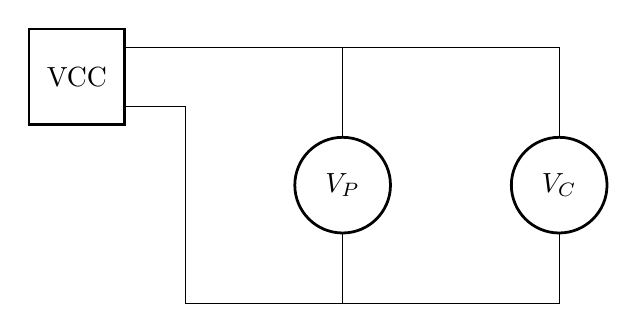
\begin{tikzpicture}[transform shape]
	% Paths, nodes and wires:
	\node[shape=rectangle, draw, line width=1pt, minimum width=1.215cm, minimum height=1.215cm] at (3.625, 7.125){} node[anchor=center, align=center, text width=0.827cm, inner sep=6pt] at (3.625, 7.125){VCC};
	\node[shape=circle, draw, line width=1pt, minimum width=1.215cm](N1) at (7, 5.75){} node[anchor=center] at (N1.text){$V_P$};
	\node[shape=circle, draw, line width=1pt, minimum width=1.215cm](N2) at (9.75, 5.75){} node[anchor=center] at (N2.text){$V_C$};
	\draw (4.25, 7.5) -| (7, 6.375);
	\draw (7, 7.5) -| (9.75, 6.375);
	\draw (9.75, 5.125) |- (9.75, 4.25) |- (7, 4.25) -| (7, 5.125);
	\draw (7, 4.25) |- (5, 4.25) -| (5, 6.5) |- (4.25, 6.75);
\end{tikzpicture}
\begingroup
\renewcommand{\figurename}{Circuito}
\caption{Experimento 1.}
\label{circuito1}
\endgroup
\end{figure}

Luego en base a los $\Delta V$ calculados, armaremos una gráfica de correción para saber cuanto se debe corregir el valor obtenido en el multímetro digital para cada valor del voltímetro analógico. Una vez obtenida la gráfica, calcularemos el indice de calse y comprobaremos si esta tiene coherencia con la indicada en la hoja de datos del instrumento.

\section{Resultados}


\begin{table}[H]
\begingroup
\renewcommand{\tablename}{Tabla}
\caption{Valores medidos y variación máxima para el experimento 1.}
\label{tabla1}
\endgroup
\resizebox{\columnwidth}{!}{%
\begin{tabular}{|c|c|c|c|c|c|c|c|}
\hline
\rowcolor[HTML]{FFCE93} 
$V_L$                                                & 1 & 2 & 3 & 4 & 5 & 6 & 7 \\ \hline
\cellcolor[HTML]{FFCCC9}$V_P$ (Pasada hacia arriba) &   &   &   &   &   &   &   \\ \hline
\cellcolor[HTML]{FFCCC9}$V_P$ (Pasada hacia abajo)  &   &   &   &   &   &   &   \\ \hline
\cellcolor[HTML]{FFCCC9}$\Delta V$ (mayor valor)     &   &   &   &   &   &   &   \\ \hline
\end{tabular}%
}
\end{table}

\begin{table}[H]
\begin{center}

\resizebox{5.5cm}{0.9cm}{%
\begin{tabular}{|c|c|c|c|c|c|c|c|}
\hline
\rowcolor[HTML]{FFCE93} 
8 & 9 & 10 & 11 & 12 & 13 & 14 & 15 \\ \hline
  &   &    &    &    &    &    &    \\ \hline
  &   &    &    &    &    &    &    \\ \hline
  &   &    &    &    &    &    &    \\ \hline
\end{tabular}%
}
\end{center}
\end{table}

\begin{figure}[H]
\centering
\resizebox{10cm}{5cm}{%
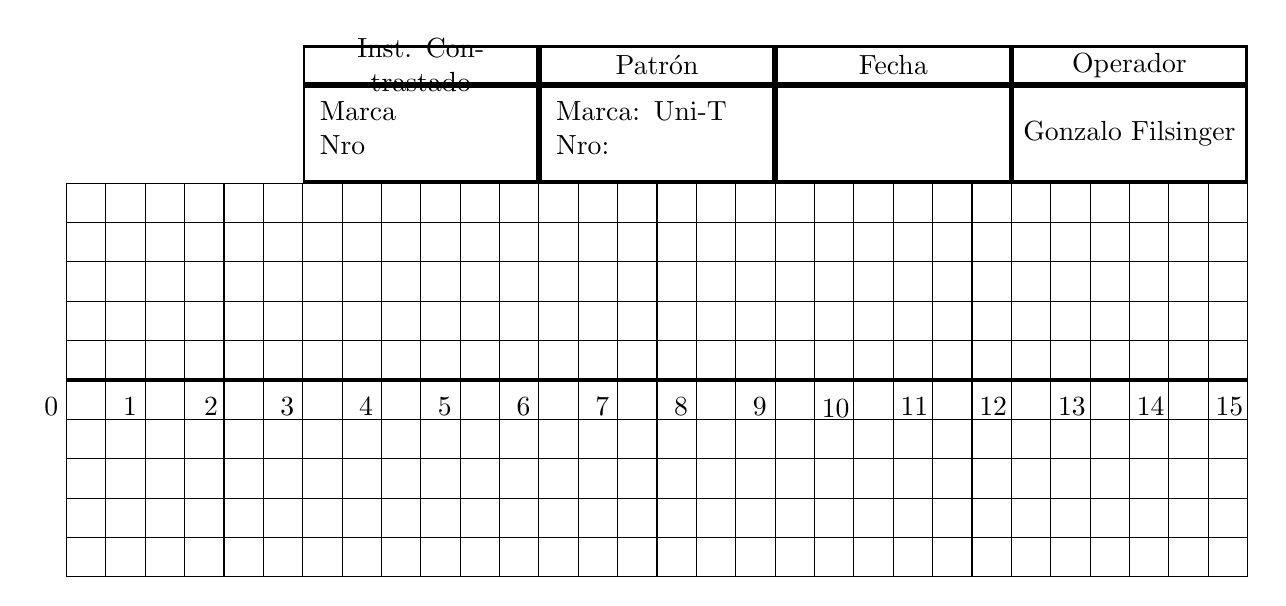
\begin{tikzpicture}[transform shape]
	% Paths, nodes and wires:
	\node[shape=rectangle, draw, line width=1pt, minimum width=2.965cm, minimum height=0.465cm] at (6.5, 9.5){} node[anchor=center, align=center, text width=2.711cm, inner sep=4.1pt] at (6.5, 9.5){Inst. Contrastado};
	\node[shape=rectangle, draw, line width=1pt, minimum width=2.965cm, minimum height=0.465cm] at (9.5, 9.5){} node[anchor=center, align=center, text width=2.577cm, inner sep=6pt] at (9.5, 9.5){Patrón};
	\node[shape=rectangle, draw, line width=1pt, minimum width=2.965cm, minimum height=0.465cm] at (12.5, 9.5){} node[anchor=center, align=center, text width=2.577cm, inner sep=6pt] at (12.5, 9.5){Fecha};
	\node[shape=rectangle, draw, line width=1pt, minimum width=2.965cm, minimum height=0.465cm] at (15.5, 9.5){} node[anchor=center, align=center, text width=2.577cm, inner sep=6pt] at (15.5, 9.5){Operador};
	\node[shape=rectangle, draw, line width=1pt, minimum width=2.965cm, minimum height=1.215cm] at (6.5, 8.625){} node[anchor=north west, align=left, text width=2.577cm, inner sep=6pt] at (5, 9.25){Marca\\Nro};
	\node[shape=rectangle, draw, line width=1pt, minimum width=2.965cm, minimum height=1.215cm] at (9.5, 8.625){} node[anchor=north west, align=left, text width=2.577cm, inner sep=6pt] at (8, 9.25){Marca: Uni-T\\Nro:};
	\node[shape=rectangle, draw, line width=1pt, minimum width=2.965cm, minimum height=1.215cm] at (12.5, 8.625){};
	\node[shape=rectangle, draw, line width=1pt, minimum width=2.965cm, minimum height=1.215cm] at (15.5, 8.625){} node[anchor=west, align=left, text width=2.711cm, inner sep=4.1pt] at (14, 8.625){Gonzalo Filsinger};
	\draw (6, 8) -- (6, 3);
	\draw (6.5, 8) -- (6.5, 3);
	\draw (2, 3) -| (17, 3);
	\draw (2, 5) -| (17, 5);
	\draw (2, 4.5) -| (17, 4.5);
	\draw (2, 4) -| (17, 4);
	\draw (2, 3.5) -| (17, 3.5);
	\draw (2, 6) -| (17, 6);
	\draw[line width=1.5pt] (2, 5.5) -| (17, 5.5);
	\draw (2, 6.5) -| (17, 6.5);
	\draw (2, 7) -| (17, 7);
	\draw (2, 7.5) -| (17, 7.5);
	\draw (2, 8) -| (17, 8);
	\draw (7, 8) -- (7, 3);
	\draw (7.5, 8) -- (7.5, 3);
	\draw (8, 8) -- (8, 3);
	\draw (8.5, 8) -- (8.5, 3);
	\draw (9, 8) -- (9, 3);
	\draw (9.5, 8) -- (9.5, 3);
	\draw (10, 8) -- (10, 3);
	\draw (10.5, 8) -- (10.5, 3);
	\draw (11, 8) -- (11, 3);
	\draw (11.5, 3) -- (11.5, 8);
	\draw (12, 8) -- (12, 3);
	\draw (12.5, 3) -- (12.5, 8);
	\draw (13, 8) -- (13, 3);
	\draw (13.5, 3) -- (13.5, 8);
	\draw (14, 8) -- (14, 3);
	\draw (14.5, 3) -- (14.5, 8);
	\draw (15, 8) -- (15, 3);
	\draw (15.5, 3) -- (15.5, 8);
	\draw (16, 8) -- (16, 3);
	\draw (16.5, 3) -- (16.5, 8);
	\draw (17, 8) -- (17, 3);
	\draw (5.5, 3) -- (5.5, 8);
	\draw (5, 8) -- (5, 3);
	\draw (4.5, 3) -- (4.5, 8);
	\draw (4, 8) -- (4, 3);
	\draw (3.5, 3) -- (3.5, 8);
	\draw (3, 8) -- (3, 3);
	\draw (2.5, 3) -- (2.5, 8);
	\draw (2, 8) -- (2, 3);
	\node[shape=rectangle, minimum width=0.465cm, minimum height=0.465cm] at (1.75, 5.25){} node[anchor=north west, align=left, text width=0.077cm, inner sep=6pt] at (1.5, 5.5){0};
	\node[shape=rectangle, minimum width=0.465cm, minimum height=0.465cm] at (2.75, 5.25){} node[anchor=north west, align=left, text width=0.077cm, inner sep=6pt] at (2.5, 5.5){1};
	\node[shape=rectangle, minimum width=0.436cm, minimum height=0.465cm] at (3.765, 5.25){} node[anchor=north west, align=left, text width=0.047cm, inner sep=6pt] at (3.529, 5.5){2};
	\node[shape=rectangle, minimum width=0.465cm, minimum height=0.465cm] at (4.75, 5.25){} node[anchor=north west, align=left, text width=0.077cm, inner sep=6pt] at (4.5, 5.5){3};
	\node[shape=rectangle, minimum width=0.465cm, minimum height=0.465cm] at (5.75, 5.25){} node[anchor=north west, align=left, text width=0.077cm, inner sep=6pt] at (5.5, 5.5){4};
	\node[shape=rectangle, minimum width=0.465cm, minimum height=0.465cm] at (6.75, 5.25){} node[anchor=north west, align=left, text width=0.077cm, inner sep=6pt] at (6.5, 5.5){5};
	\node[shape=rectangle, minimum width=0.465cm, minimum height=0.465cm] at (7.75, 5.25){} node[anchor=north west, align=left, text width=0.077cm, inner sep=6pt] at (7.5, 5.5){6};
	\node[shape=rectangle, minimum width=0.465cm, minimum height=0.465cm] at (8.75, 5.25){} node[anchor=north west, align=left, text width=0.077cm, inner sep=6pt] at (8.5, 5.5){7};
	\node[shape=rectangle, minimum width=0.465cm, minimum height=0.465cm] at (9.75, 5.25){} node[anchor=north west, align=left, text width=0.077cm, inner sep=6pt] at (9.5, 5.5){8};
	\node[shape=rectangle, minimum width=0.465cm, minimum height=0.465cm] at (10.75, 5.25){} node[anchor=north west, align=left, text width=0.077cm, inner sep=6pt] at (10.5, 5.5){9};
	\node[shape=rectangle, minimum width=0.715cm, minimum height=0.436cm] at (11.75, 5.235){} node[anchor=north west, align=left, text width=0.327cm, inner sep=6pt] at (11.375, 5.471){10};
	\node[shape=rectangle, minimum width=0.715cm, minimum height=0.465cm] at (12.75, 5.25){} node[anchor=north west, align=left, text width=0.327cm, inner sep=6pt] at (12.375, 5.5){11};
	\node[shape=rectangle, minimum width=0.715cm, minimum height=0.465cm] at (13.75, 5.25){} node[anchor=north west, align=left, text width=0.327cm, inner sep=6pt] at (13.375, 5.5){12};
	\node[shape=rectangle, minimum width=0.715cm, minimum height=0.465cm] at (14.75, 5.25){} node[anchor=north west, align=left, text width=0.327cm, inner sep=6pt] at (14.375, 5.5){13};
	\node[shape=rectangle, minimum width=0.715cm, minimum height=0.465cm] at (15.75, 5.25){} node[anchor=north west, align=left, text width=0.327cm, inner sep=6pt] at (15.375, 5.5){14};
	\node[shape=rectangle, minimum width=0.715cm, minimum height=0.465cm] at (16.75, 5.25){} node[anchor=north west, align=left, text width=0.327cm, inner sep=6pt] at (16.375, 5.5){15};
\end{tikzpicture}%
}
\begingroup
\renewcommand{\figurename}{Gráfico}
\setcounter{figure}{0}
\caption{Tabla de corrección.}
\label{grafico1}
\endgroup
\end{figure}

\section{Conclusión}
Se logró verificar que...

% Referencias bibliográficas
\begin{thebibliography}{1}
\bibitem{IEEEhowto:kopka}
TP1 version definitiva V 02 2026 Medidas Electrónicas I
\end{thebibliography}

\end{document}